\documentclass{VUMIFPSkursinis}
\usepackage{algorithmicx}
\usepackage{algorithm}
\usepackage{algpseudocode}
\usepackage{amsfonts}
\usepackage{amsmath}
\usepackage{bm}
\usepackage{caption}
\usepackage{color}
\usepackage{float}
\usepackage{graphicx}
\usepackage{listings}
\usepackage{subfig}
\usepackage{wrapfig}
\usepackage{pdflscape} %Keep it to pdflscape or I can't rotate my diagram (K.S.)
\usepackage{longtable}
\usepackage[table]{xcolor}
\usepackage{multirow}
\usepackage[usestackEOL]{stackengine}
\usepackage{longtable}
\usepackage{subfig}
\usepackage{wrapfig}


\usepackage{enumitem}
%PAKEISTA, tarpai tarp sąrašo elementų
\setitemize{noitemsep,topsep=0pt,parsep=0pt,partopsep=0pt}
\setenumerate{noitemsep,topsep=0pt,parsep=0pt,partopsep=0pt}

% Titulinio aprašas
\university{Vilniaus universitetas}
\faculty{Matematikos ir informatikos fakultetas}
\department{Programų sistemų katedra}
\papertype{Programų sistemų inžinerijos laboratorinis darbas Nr. 3}
\title{Kavinės staliuko rezervavimo aplikacija}
\titleineng{Cafe table rezervation app}
\status{2 kurso 5 grupės studentai}
\author{Paulius Grigaliūnas}
\secondauthor{Karolis Staskevičius}
\thirdauthor{Modestas Dulevičius}
\fourthauthor{Albert Jurkoit}
\fifthauthor{Šarūnas Kazimieras Buteikis}
     

% \secondauthor{Vardonis Pavardonis}   % Pridėti antrą autorių
\supervisor{dr. Vytautas Valaitis}
\date{Vilnius – \the\year}

% Nustatymai
% \setmainfont{Palemonas}   % Pakeisti teksto šriftą į Palemonas (turi būti įdiegtas sistemoje)

\begin{document}
% PAKEISTA	
\maketitle
\cleardoublepage\pagenumbering{arabic}
\setcounter{page}{2}


%ANOTACIJA

\sectionnonum{ANOTACIJA}
\noindent


%TURINYS(TOC)
\tableofcontents

%ĮVADAS
\sectionnonum{Įvadas}
\noindent

\section{Verslo proceso aprašas}

\section{Išorinė analizė}

\section{Vidinė proceso analizė}

Šiame skyriuje atliekama vidinė verslo proceso analizė, siekiant nustatyti kavinės rezervavimo programėles stiprybes ar silpnybes, kylančias iš paties verslo proceso (ne jo aplinkos).\\\\

\subsection{Pagrindinės dalykinės srities esybės}
\noindent \textbf{Kavinė} - maitinimo paskirties įstaiga.\\
\textbf{Kavinės} savininkas -asmuo, kuriam priklauso kavinė.\\
\textbf{Klientas} - asmuo, rezervavęs staliuką. \\
\textbf{Maisto tiekėjas} - įmonė, iš kurios kavinė gauna reikalingas prekes ir produktus. \\
\textbf{Rezervacija} - nutarimas, leidžiantis klientui iš anksto turėti konkretų staliuką tam tikru laiku. \\
\textbf{Staliukas} - vieta, prie kurios klientas sėdi restorane.\\
\textbf{Virtuvė} - vieta, kurioje yra ruošiamas užsakymas kavinėje.\\
\textbf{Sąskaita} - kliento apmokėjimas už užsakymą.\\
\textbf{Darbuotojas} - asmuo, kuris dirba kavinėje ir už tai gauna algą.\\

\begin{landscape}
\subsection{Dalykinės srities statinė struktūra}

	\begin {figure}[H]
	\centering
		\caption{Dalykinės srities statinė struktūra}
		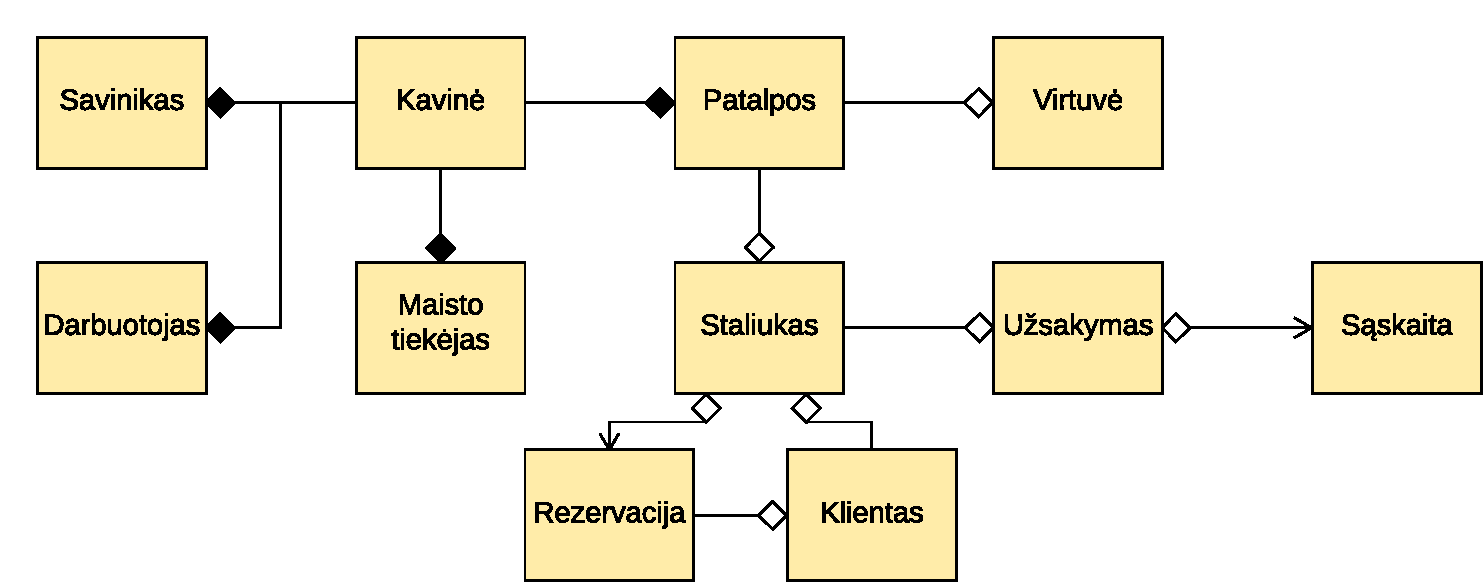
\includegraphics[scale=1]{img/3lab/Diagrama1}
		
		\label{fig:ER}
	\end{figure}
\end{landscape}

Kavinė negali egzistuoti be maisto tiekėjų (nebus iš ko ruošti maistą) ir be darbuotojų (nebus galima efektyviai aptarnauti klientų), tad šios esybės sudaro kompoziciją, nes viena negali veikti be kitos.\\
Kavinė gali vykti ir be patalpų, kadangi kavinės staliukai gali stovėti ir 
lauke , todėl šie komponentai sudaro agregaciją.\\
Prie  staliuko  neprivalo  sėdėti  klientas,  nes
staliukas  yra  tik  priemonė  aptarnauti ir jam patogiai jaustis restorane,
klientą.Staliukas taip pat gali nebūti rezervuotas, todėl šios esybės sudaro agregaciją.\\
Patalpose gali būti staliukai ir virtuvė, tačiau tai nėra būtina sąlyga, todėl tai sudaro 
agregaciją.\\
Užsakymas konkretizuoja esybę staliukas.\\
Sąskaita seka po to, kai atliekamas užsakymas.\\

\subsection{Užduočių diagrama}
Klientai  yra  agentai,  kurie  naudodamiesi  kavinės  teikiamomis 
paslaugomis  įgyvendina  užduotis - palydėti  atsisėda  prie  staliuko,  atlieka  užsakymus  ir  juos apmoka. \\
Darbuotojas yra agentas, kuris atlieka tokias užduotis kaip palydėti klientą prie staliuko, 
priimti užsakymą, jį paruošti ir priimti apmokėjimą.\\
Tiekėjai yra agentai, kurių užduotis yra pristatyti reikalingas prekes ir produktus kavinei.


\subsection{Užduočių vykdymo scenarijai}

\subsection{Dalykinės srities dinaminė struktūra}

\section{Analizės rezultatai}

\section{Verslo proceso tobulinimo strategija}

\section{Sistemos naudojimo scenarijai}

\section{Įgyvendinamumo ir naudos analizė}

\section{Literatūros sąrašas}


\end{document}
